%=========================================================================
% Entrega 6 - PF3325 Redes
% Detection of Phishing Websites Using Artificial Neural Networks
% IEEE conference (two-column) format. Compile with pdflatex + bibtex:
%   pdflatex main ; bibtex main ; pdflatex main ; pdflatex main
%=========================================================================
\documentclass[conference]{IEEEtran}
\IEEEoverridecommandlockouts

\usepackage{cite}
\usepackage{amsmath,amssymb,amsfonts}
\usepackage{graphicx}
\usepackage{textcomp}
\usepackage{xcolor}
\usepackage{booktabs}
\usepackage{array}
\usepackage{url}
\usepackage[hidelinks]{hyperref}

\graphicspath{{figures/}}

\begin{document}

\title{Detection of Phishing Websites Using Artificial\\Neural Networks with a Real-Time Detection Service}

\author{
  \IEEEauthorblockN{Gabriel Fallas}
  \IEEEauthorblockA{\textit{Escuela de Ciencias de la Computaci\'on e Inform\'atica} \\
    \textit{Universidad de Costa Rica}\\
    San Jos\'e, Costa Rica \\
    gabriel.fallas@ucr.ac.cr}
  \and
  \IEEEauthorblockN{Valeria Chinchilla}
  \IEEEauthorblockA{\textit{Escuela de Ciencias de la Computaci\'on e Inform\'atica} \\
    \textit{Universidad de Costa Rica}\\
    San Jos\'e, Costa Rica \\
    valeria.chinchilla@ucr.ac.cr}
}

\maketitle

\begin{abstract}
Phishing remains one of the most damaging cybersecurity threats, with the
Anti-Phishing Working Group recording 4.8 million attacks in 2024. Blacklists
and hand-written heuristics are inherently reactive and fail against sites that
live for only a few hours. We present an end-to-end phishing detection system
built on the UCI Phishing Websites dataset (11,055 instances, 30 features). We
train a regularized Multilayer Perceptron (MLP) using Batch Normalization,
Dropout, $L_2$ regularization and Early Stopping, and compare it against Random
Forest and Support Vector Machine baselines. On a held-out, stratified test set
the MLP reaches 96.5\% accuracy, 98.8\% recall and an AUC of 0.994, with the
highest recall of all evaluated models---the most important property for a
security filter. Beyond offline classification, we contribute a real-time
detection service: a feature extractor that derives the dataset features from a
raw URL using the URL string, the fetched HTML/JavaScript, DNS and WHOIS, served
through a FastAPI REST API with an interactive web demo. We openly discuss the
limitations of real-time extraction caused by services (Alexa, Google PageRank)
that no longer exist. The deployable detection component is, to our knowledge,
absent from the foundational works on this dataset.
\end{abstract}

\begin{IEEEkeywords}
phishing detection, neural networks, multilayer perceptron, machine learning,
cybersecurity, URL classification, real-time inference, REST API
\end{IEEEkeywords}

%=========================================================================
\section{Introduction}
%=========================================================================
Phishing is a form of social engineering in which an attacker builds a
fraudulent website that imitates a legitimate one to trick users into revealing
credentials, financial details or personal data~\cite{mohammad2012}. The scale
of the problem is substantial: the Anti-Phishing Working Group (APWG) recorded
4.8 million phishing attacks during 2024---the highest annual total since the
organization was founded in 2003---and related Business Email Compromise losses
exceeded USD~2.8 billion in the United States alone~\cite{apwg2024q4}.

Two classical defensive paradigms dominate practice. \emph{Blacklist}-based
systems such as Google Safe Browsing keep databases of known malicious URLs.
While effective against previously reported sites, they are fundamentally
reactive: a phishing page may be operational for fewer than 24 hours before it
is reported, listed and taken down, during which thousands of victims can be
deceived. \emph{Heuristic}-based systems encode expert rules---e.g. ``if the URL
contains an IP address, flag it''---but require constant manual maintenance and
are easily evaded once attackers learn the rule set.

Machine learning offers an attractive alternative: instead of hand-coding rules,
a model learns discriminative patterns directly from labeled data. This paper
investigates Multilayer Perceptron (MLP) neural networks for phishing detection
on the UCI Phishing Websites dataset~\cite{uci327}. Our contributions are:

\begin{enumerate}
  \item A regularized MLP trained and evaluated against Random Forest and SVM
        baselines under an identical preprocessing and split protocol, with a
        focus on \emph{recall} as the security-critical metric.
  \item A \textbf{real-time detection service}: a feature extractor that turns a
        raw URL into the 30 dataset features in real time, wrapped in a FastAPI
        REST API with an interactive web demo---a deployable component absent
        from the foundational works on this dataset.
  \item An honest analysis of the practical limits of real-time feature
        extraction, caused by third-party services used to build the original
        dataset that are now defunct.
\end{enumerate}

The remainder of the paper is organized as follows. Section~\ref{sec:related}
reviews related work. Section~\ref{sec:background} summarizes the theoretical
background. Section~\ref{sec:method} describes the methodology, and
Section~\ref{sec:impl} the real-time implementation. Section~\ref{sec:results}
reports results and analysis, Section~\ref{sec:disc} discusses limitations, and
Section~\ref{sec:concl} concludes.

%=========================================================================
\section{Related Work}\label{sec:related}
%=========================================================================
Research on automated phishing detection spans more than fifteen years and has
evolved from early neural networks to modern deep learning.
Table~\ref{tab:related} summarizes the most relevant prior work.

\begin{table}[t]
\caption{Comparison of related works}
\label{tab:related}
\centering
\renewcommand{\arraystretch}{1.2}
\setlength{\tabcolsep}{3pt}
\begin{tabular}{@{}lcccc@{}}
\toprule
\textbf{Reference} & \textbf{Technique} & \textbf{Size} & \textbf{Best Acc.} & \textbf{Real-time} \\
\midrule
Mohammad '12~\cite{mohammad2012} & Feature eng. & 2{,}500 & 84\% & No \\
Mohammad '14~\cite{mohammad2014} & J48/RF/SSNN & 11{,}055 & $\sim$97\% & No \\
Sahingoz '19~\cite{sahingoz2019}  & RF + NLP    & 73{,}575 & 97.3\% & No \\
Vrban\v{c}i\v{c} '20~\cite{vrbancic2020} & XGBoost & 88{,}647 & $\sim$97.6\% & No \\
Chatterjee '19~\cite{chatterjee2019} & Deep RL & Custom & $\sim$96\% & No \\
\textbf{This work} & \textbf{MLP+RF+SVM} & \textbf{11{,}055} & \textbf{97.2\%} & \textbf{Yes} \\
\bottomrule
\end{tabular}
\end{table}

A distinction often overlooked concerns the two foundational papers by Mohammad
\emph{et~al.} The 2012 paper~\cite{mohammad2012} is primarily a \emph{feature
engineering} exercise: the authors designed and validated automated extraction
rules for 17 URL and page characteristics using JavaScript and PHP, evaluated on
2,500 URLs from PhishTank. No production classifier was trained; the
contribution was a validated feature set and its extraction methodology. The
2014 paper~\cite{mohammad2014} expanded the dataset to 11,055 samples and 30
features and compared several classifiers, including a Self-Structuring Neural
Network (SSNN) that reached roughly 97\% accuracy---the direct predecessor of
our work and our primary neural baseline.

Sahingoz \emph{et~al.}~\cite{sahingoz2019} added Natural Language Processing
features computed from the URL string (character $n$-grams and token attributes)
and reached 97.32\% with Random Forest on 73,575 URLs, showing that feature
richness matters beyond classifier choice. Vrban\v{c}i\v{c}
\emph{et~al.}~\cite{vrbancic2020} released larger benchmark datasets and
established ensemble methods (XGBoost, Random Forest, $\sim$97.6\%) as the
dominant classical paradigm. Chatterjee and Namin~\cite{chatterjee2019} explored
Deep Reinforcement Learning, which adapts to evolving tactics at the cost of
training complexity.

\textbf{Gap addressed.} A consistent limitation across these works is the
absence of a deployable, real-time detection component: each treats phishing
detection as an offline experiment---train, evaluate on a held-out set, report
metrics---without exposing the classifier as a service that scores an arbitrary
new URL on demand. Our work closes this gap with a complete real-time pipeline
while keeping a rigorous offline comparison.

%=========================================================================
\section{Theoretical Background}\label{sec:background}
%=========================================================================
\subsection{Phishing Attack Vectors}
Phishing attacks are commonly grouped into three vectors. \emph{URL-based}
attacks manipulate the domain name through typosquatting (e.g.
\texttt{paypa1.com}), Unicode homograph characters, or raw IP addresses that
bypass domain filtering. \emph{Content-based} attacks replicate the visual
appearance of a legitimate site and host a form that exfiltrates submitted data.
\emph{DNS-based} attacks redirect legitimate domain names through DNS spoofing.
The 30 dataset features capture both URL structural properties and
HTML/JavaScript behavioral signals, so our approach targets the first two
vectors.

\subsection{The UCI Phishing Websites Dataset}
The dataset~\cite{uci327} contains 11,055 instances labeled phishing ($-1$) or
legitimate ($1$), described by 30 features in four
categories~\cite{mohammad2014}: \emph{Address-Bar based} (12 features: IP
address, URL length, shortening service, \texttt{@} symbol, double-slash
redirect, prefix/suffix, subdomain count, SSL state, registration length,
favicon origin, port, HTTPS token); \emph{Abnormal based} (6: request URL,
anchor URLs, links in tags, server-form handler, email submission, abnormal
URL); \emph{HTML/JavaScript based} (5: redirects, \texttt{onmouseover},
right-click, pop-ups, \texttt{iframe}); and \emph{Domain based} (7: domain age,
DNS record, web traffic, PageRank, Google index, inbound links, statistical
reports). Each feature uses a ternary encoding---$1$ (legitimate), $0$
(suspicious), $-1$ (phishing)---which carries more information than a binary
flag. The class split is near-balanced (55.7\% legitimate, 44.3\% phishing), so
no special imbalance handling is required.

\subsection{Multilayer Perceptron}
An MLP is a feedforward network with an input layer, one or more hidden layers,
and an output layer~\cite{lecun2015}. Hidden units use the ReLU activation
$\mathrm{ReLU}(z)=\max(0,z)$, which mitigates vanishing gradients. The output is
a single sigmoid unit producing $p\in[0,1]$, the probability that the URL is
legitimate. Weights are learned by minimizing the binary cross-entropy loss
\begin{equation}
\mathcal{L}(y,p) = -\bigl[y\log p + (1-y)\log(1-p)\bigr],
\end{equation}
with the Adam optimizer and backpropagation. To control overfitting we combine
\emph{Dropout}~\cite{srivastava2014} (randomly zeroing units during training),
\emph{Batch Normalization}~\cite{ioffe2015} (normalizing pre-activations per
mini-batch), $L_2$ weight penalties, and \emph{Early Stopping} on validation
loss.

%=========================================================================
\section{Methodology}\label{sec:method}
%=========================================================================
Fig.~\ref{fig:pipeline} shows the complete system. An offline lane trains and
persists the model; a real-time lane reuses the persisted artifacts to score new
URLs.

\begin{figure}[t]
\centering
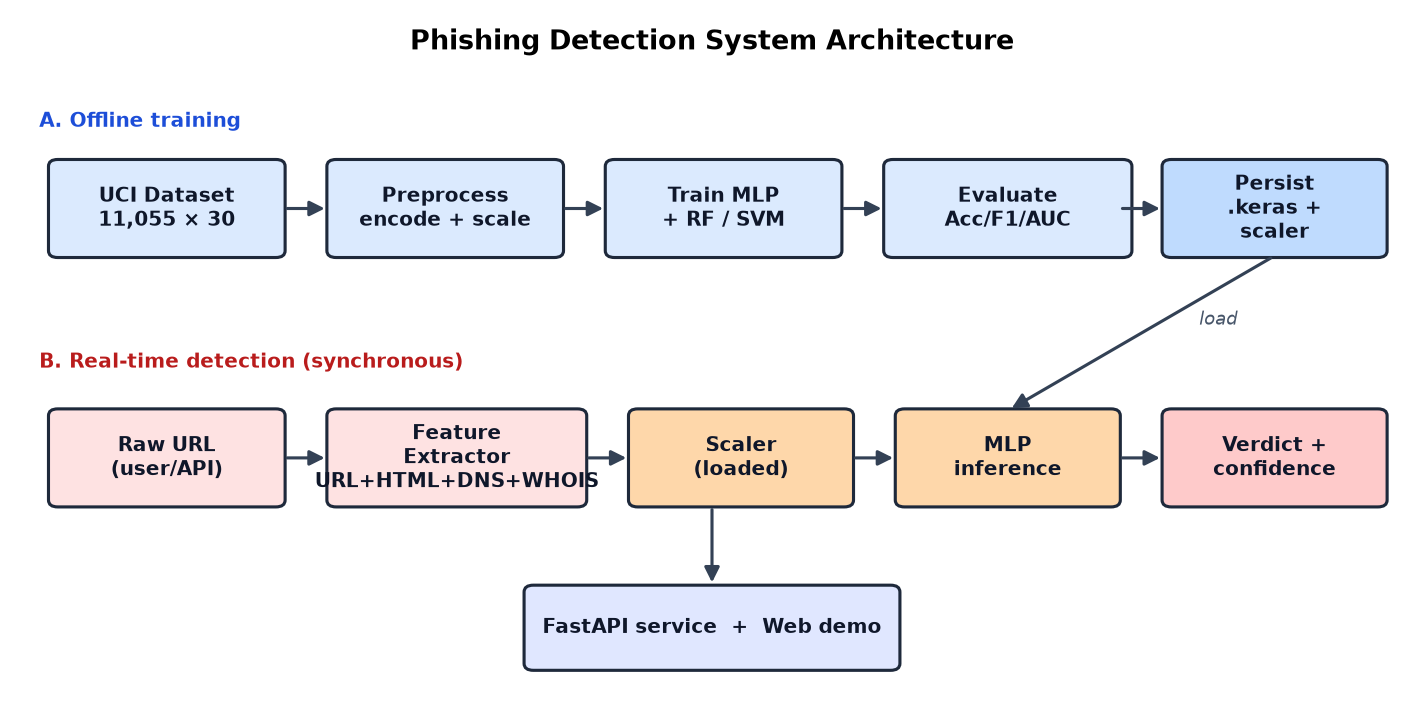
\includegraphics[width=\columnwidth]{fig_pipeline.png}
\caption{End-to-end architecture: offline training (top) and real-time
synchronous detection (bottom) sharing the persisted model and scaler.}
\label{fig:pipeline}
\end{figure}

\subsection{Preprocessing}
The target $\mathit{Result}\in\{-1,1\}$ is mapped to $\{0,1\}$ for the sigmoid
output. Features keep their ternary encoding, since the intermediate $0$
(suspicious) value is informative. All 30 features are standardized with
\texttt{StandardScaler} fit \emph{only} on the training split to avoid leakage.
The data is partitioned by stratified splitting into 70\% training (7,737), 15\%
validation (1,659) and 15\% test (1,659).

\subsection{Classifiers}
Two classical baselines are trained: a Random Forest of 100 trees and an SVM
with an RBF kernel. The proposed network, shown in Fig.~\ref{fig:mlp}, is
\begin{center}
\small
Input(30)$\rightarrow$Dense(128)+BN+ReLU+Drop(0.3)$\rightarrow$\\
Dense(64)+BN+ReLU+Drop(0.2)$\rightarrow$Dense(32)+ReLU+Drop(0.1)\\
$\rightarrow$Dense(1, sigmoid),
\end{center}
with $L_2$ regularization ($\lambda=10^{-3}$), Adam (learning rate $10^{-3}$),
binary cross-entropy loss, and Early Stopping (patience 10) restoring the best
weights. The network has 15,105 trainable parameters.

\begin{figure}[t]
\centering
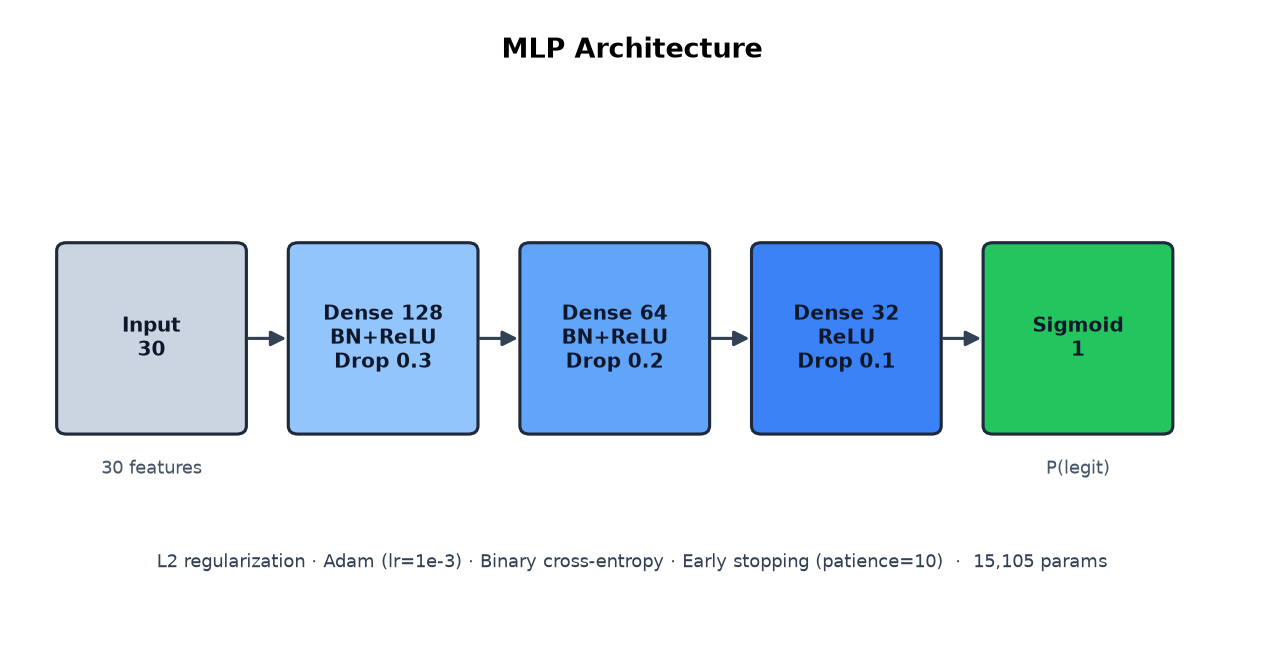
\includegraphics[width=\columnwidth]{fig_mlp.png}
\caption{Proposed MLP. Batch Normalization and Dropout follow the first two
dense layers; a single sigmoid unit outputs $P(\text{legitimate})$.}
\label{fig:mlp}
\end{figure}

%=========================================================================
\section{Real-Time Detection Implementation}\label{sec:impl}
%=========================================================================
The real-time component is the main engineering contribution. It turns a raw URL
into a verdict in a single synchronous request.

\subsection{Feature Extractor}
Given a URL, the extractor computes the 30 features in the exact training order.
Features grounded in observable data are measured directly:
\begin{itemize}
  \item \emph{URL string}: IP-address host, length bands, shortening services,
        \texttt{@} symbol, double-slash redirect, prefix/suffix, subdomain
        depth, and embedded HTTPS token---parsed with \texttt{tldextract}.
  \item \emph{Transport}: the SSL final state is checked through a real TLS
        handshake; redirects are counted from the HTTP response chain.
  \item \emph{HTML/JavaScript}: the page is fetched and parsed with
        BeautifulSoup to compute the fraction of external request URLs, anchors,
        and links in tags, the server-form handler, email submission, and the
        \texttt{onmouseover}, right-click, pop-up and \texttt{iframe} signals.
  \item \emph{Network}: DNS A/AAAA records are resolved; WHOIS provides domain
        age and registration length.
\end{itemize}

\subsection{Honest Limits of Real-Time Extraction}
Four features depend on services that no longer offer a free public interface:
\emph{web\_traffic} (Alexa, retired May 2022), \emph{Page\_Rank} (Toolbar
PageRank, retired 2016), \emph{Links\_pointing\_to\_page} (backlink index), and
\emph{Statistical\_report}/\emph{Google\_Index} (search/threat-intel APIs). For
these the extractor returns a neutral default and \emph{records the provenance}
of every feature as \texttt{measured} or \texttt{default}, so the service is
transparent about how much of a verdict rests on live evidence. In a typical run
against a reachable site, 24 of 30 features are measured live.

\subsection{REST API and Demo}
The trained model (\texttt{best\_model.keras}) and scaler
(\texttt{scaler.joblib}) are served by a FastAPI application with three
endpoints: \texttt{POST /predict/features} (score a 30-value vector),
\texttt{POST /predict/url} (extract and score a raw URL, returning the verdict,
confidence and per-feature provenance), and \texttt{GET /} (an interactive web
demo). Inference is sub-second once the model is loaded.

%=========================================================================
\section{Results and Analysis}\label{sec:results}
%=========================================================================
All models are evaluated on the same stratified test set of 1,659 samples.
Table~\ref{tab:results} reports the metrics.

\begin{table}[t]
\caption{Test-set performance (1{,}659 samples)}
\label{tab:results}
\centering
\renewcommand{\arraystretch}{1.25}
\setlength{\tabcolsep}{4pt}
\begin{tabular}{@{}lccccc@{}}
\toprule
\textbf{Model} & \textbf{Acc.} & \textbf{Prec.} & \textbf{Recall} & \textbf{F1} & \textbf{AUC} \\
\midrule
Random Forest      & \textbf{0.972} & \textbf{0.969} & 0.981 & \textbf{0.975} & \textbf{0.996} \\
SVM (RBF)          & 0.946 & 0.935 & 0.971 & 0.953 & 0.987 \\
MLP (proposed)     & 0.965 & 0.951 & \textbf{0.988} & 0.969 & 0.994 \\
\bottomrule
\end{tabular}
\end{table}

The MLP achieves 96.5\% accuracy and an AUC of 0.994, statistically on par with
the Random Forest and clearly above the SVM. Crucially, the MLP attains the
\textbf{highest recall (98.8\%)} of all models. In a security setting recall is
the decisive metric: a false negative is a phishing site mislabeled as
legitimate that reaches the user, whereas a false positive only inconveniences a
user with a warning. The MLP confusion matrix (Fig.~\ref{fig:cm}) shows only 11
false negatives out of 924 phishing samples, versus 47 false positives---an
operating point well suited to a protective filter. The Random Forest remains a
strong, cheaper baseline and confirms that our preprocessing reproduces the
$\sim$97\% benchmark of Mohammad \emph{et~al.}~\cite{mohammad2014}.

\begin{figure}[t]
\centering
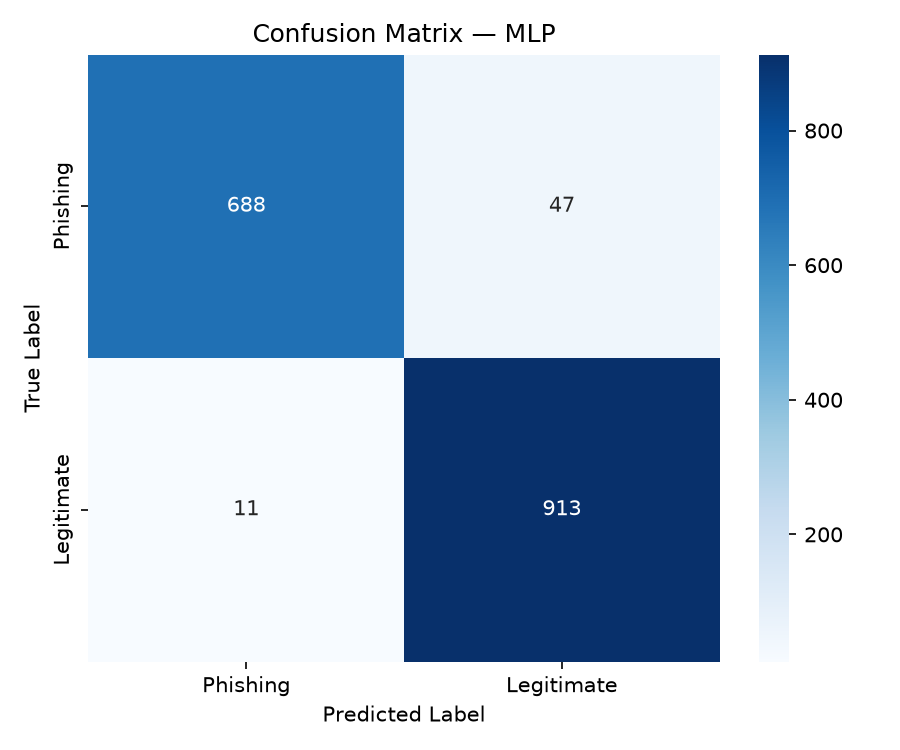
\includegraphics[width=0.82\columnwidth]{confusion_mlp.png}
\caption{MLP confusion matrix on the test set. Only 11 phishing pages
(of 924) are missed.}
\label{fig:cm}
\end{figure}

\begin{figure}[t]
\centering
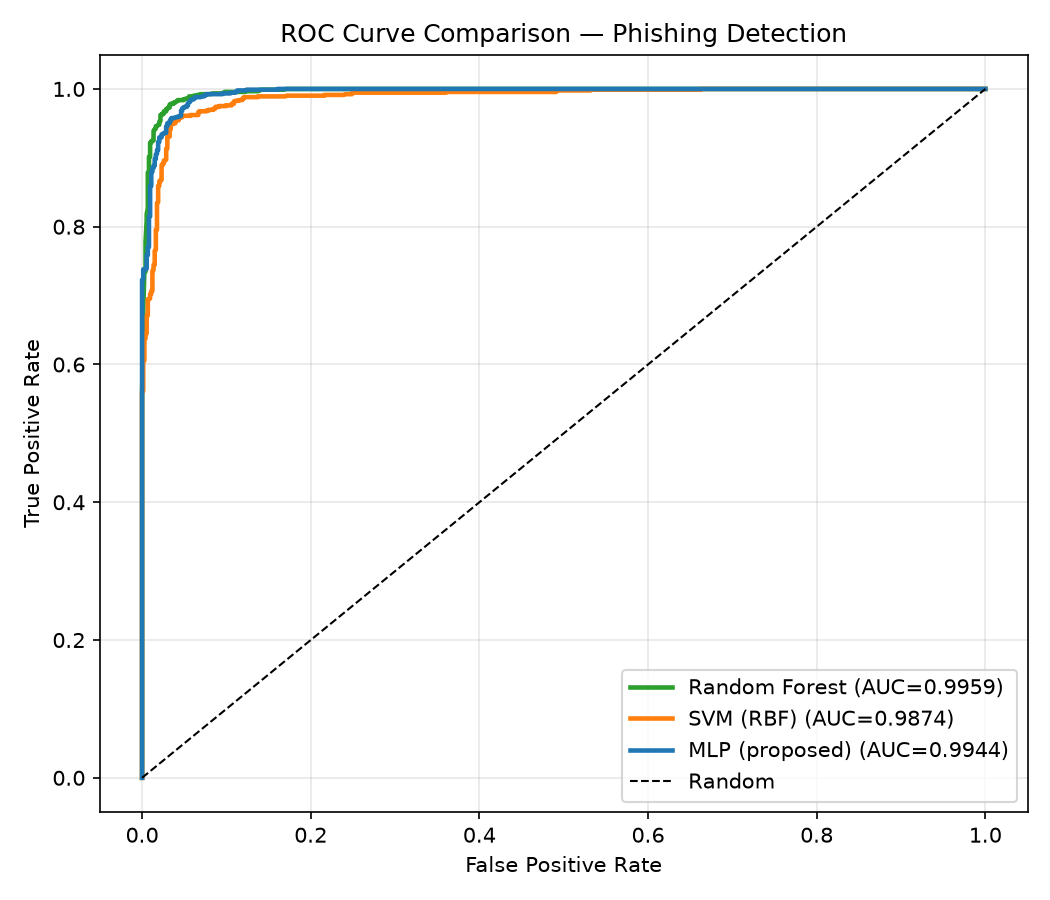
\includegraphics[width=\columnwidth]{roc_comparison.png}
\caption{ROC curves for the three classifiers. All exceed 0.98 AUC; the MLP and
Random Forest are nearly indistinguishable.}
\label{fig:roc}
\end{figure}

The ROC curves in Fig.~\ref{fig:roc} confirm that all three classifiers operate
far above the random baseline, with the MLP and Random Forest essentially
overlapping. The training history (Fig.~\ref{fig:hist}) shows stable convergence
within roughly 45 epochs and no divergence between training and validation loss,
indicating that the combination of Dropout, Batch Normalization, $L_2$ and Early
Stopping effectively controls overfitting.

\begin{figure}[t]
\centering
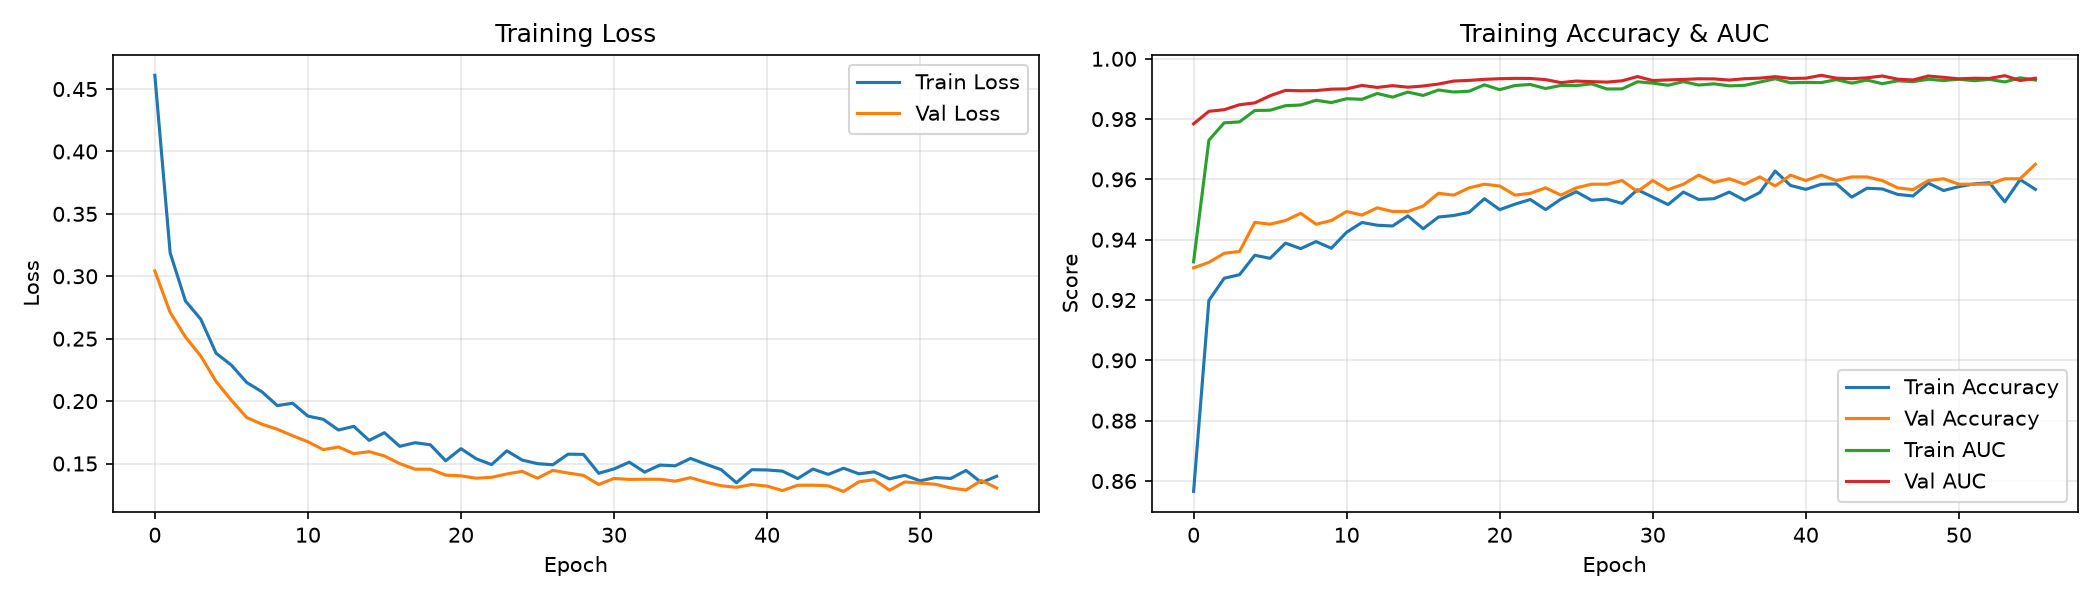
\includegraphics[width=\columnwidth]{training_history.png}
\caption{MLP training history. Validation loss tracks training loss, with Early
Stopping restoring the best epoch.}
\label{fig:hist}
\end{figure}

\subsection{End-to-End Real-Time Behavior}
On reachable, well-behaved sites the extractor measures 24 of 30 features live
and the API returns a confident, correct verdict in under a second. The
remaining six features fall back to neutral defaults. We observe the expected
failure mode when a page cannot be fetched (unreachable host, aggressive
anti-bot defenses): the number of live-measured features drops and the verdict
leans on URL-only signals, reducing confidence. This is an inherent property of
real-time extraction rather than a defect of the classifier, and the provenance
map makes it explicit to the caller.

%=========================================================================
\section{Discussion and Limitations}\label{sec:disc}
%=========================================================================
Three limitations deserve emphasis. First, the dataset, although a standard
benchmark, dates from 2014; phishing tactics have since evolved, so absolute
metrics may overstate performance on contemporary attacks. Second, several
features cannot be reproduced in real time because their source services are
defunct, creating a distribution shift between the training features and those
available at inference; our provenance mechanism surfaces this but does not
eliminate it. Third, content-based extraction requires fetching the target page,
which introduces latency and exposure to anti-scraping defenses. Future work
should retrain on a modern dataset whose features are fully reproducible online
(e.g. URL-only lexical features as in~\cite{sahingoz2019}), add caching and
asynchronous batching to the API, and explore calibrated confidence so that
low-evidence verdicts are flagged rather than reported at face value.

%=========================================================================
\section{Conclusion}\label{sec:concl}
%=========================================================================
We presented an end-to-end phishing detection system on the UCI Phishing
Websites dataset. A regularized MLP reaches 96.5\% accuracy, 98.8\% recall and
0.994 AUC, matching the Random Forest baseline while offering the best recall---
the property that matters most for a security filter. Beyond offline
classification, we built and validated a real-time detection service: a feature
extractor from raw URLs and a FastAPI REST API with a web demo, together with an
honest account of what can and cannot be measured online today. This deployable
component is the main differentiator from the foundational works on this
dataset, turning a benchmark experiment into a usable detector.

\bibliographystyle{IEEEtran}
\bibliography{references}

\end{document}
